\subsection*{Экспериментальная установка}


Свет от источника $S$ с помощью линзы фокусируется на входную щель призменного монохроматора УМ-2, выделяющего узкий спектральный интервал, и попадает на катод фотоэлемента ФЭ.
\begin{figure}[h]
    \centering
    \includegraphics[width=0.5\textwidth]{imgs/exp.png}
    \caption{Схема экспериментальной установки}
    \label{fig:exp}
\end{figure}
Фотоэлемент представляет собой откаченный до высокого вакуума стеклянный баллон, внутри которого расположены два электрода: фотокатод и анод. Фотоэлемент обладает спектральной чувствительностью в области длин волн от $300$ до $850$ нм, наибольшая чувствительность ФЭ в области от $400$ до $500$ нм. 

Фототок, протекающий в ФЭ, мал, так что для его измерения используется усилитель постоянного тока. Тормозящий потенциал регулируется, измерения осуществляются с помощью цифрового вольтметра.



\newpage


\subsection*{Измерения}

\textbf{Градуировка}. Для начала была произведена градуировка барабана монохроматора УМ-2 по спектру неоновой лампы. Прокрутка барабана допускала приводила к погрешности измерений $\Delta n \sim 15$ у.е. Таким образом былы получены данные таблицы № \ref{grad_tab}, где $n$ -- показания на барабане УМ-2 в условных единицах.



\begin{figure}[ht]
    \centering
    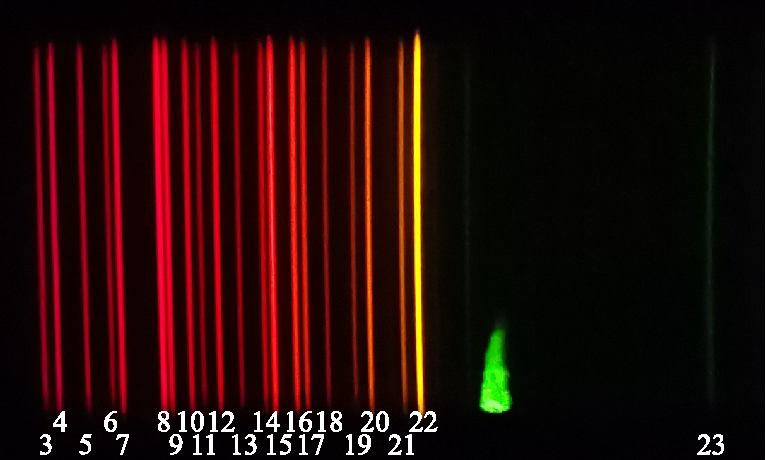
\includegraphics[width=0.4\textwidth]{figs/photo_1.pdf}
    \caption{Спектр неоновой лампы, фото на выходе из УМ-2}
    %\label{fig:}
\end{figure}


Для удобства было построено приближение функции $\lambda(n)$ (рис. \ref{fig:1}). Погрешность в $\lambda$ была оценена, как $\lambda'(n) \Delta n$, что позволило оценить $\chi^2 \approx 3.3$ для полинома второй степени, что является адекватной величиной.
\begin{equation*}
    \lambda(n) = (1.5 \pm 0.1) 10^{-4} n^2 + (-4.7 \pm 0.6) 10^{-1} n + (8.7 \pm 0.6) 10^2,
\end{equation*}
что упростило дальнейшую работу с обородованием.

\vspace{-5mm}

\begin{figure}[ht]
    \centering
    \includegraphics[width=0.5\textwidth]{figs/fig1.pdf}
    \vspace{-4mm}
    \caption{Приближение зависимости $\lambda(n)$ полиномом}
    \label{fig:1}
\end{figure}


\textbf{Зависимость фототока от катодного потенциала}. После окончания градуировки, окуляр был заменен на ФЭ, неоновая лампа заменена на электрическую лампу. После подстройки темнового тока к почти нулевым значеням, были измерены зависимости фототока ($U_1$), усиленного усилителем (по итоге снималось напряжение), от величины катодного потенциала ($U_2$). Напряжения снимались цифровыми вольтметрами, так были получены данные таблицы №\ref{tab:2}, визуализация данных на рис. \ref{fig:UU}. 

Подобная зависимость была снята на трёх различных длинах волн с максимальным разбросом по диапазону.


\begin{figure}[ht]
    \centering
    \includegraphics[width=0.55\textwidth]{figs/fig2.pdf}
    \vspace{-5mm}
    \caption{Зависимость фототока от катодного потенциала при различных длинах волн}
    \label{fig:UU}
\end{figure}




Погрешность данных была принята равной $2 \%$ от результата $+ 10$ мВ (визуальные флуктуации). Длины волн получены, на основе предыдущего пункта ($1900$ у.е. $\to 539$ нм,
$2250$ у.е. $\to 598$ нм,
$2500$ у.е. $\to 663$ нм). Темновой фототок проверялся при закрытой крышке УМ-2.